
Ultimately, our goal is to make statements about the \textit{global} relationships which exist in the graph, using information which comes to us via \textit{local} relationships between nodes.
Arrow's IIA criteria requires the consideration of local relationships only, but as we have seen, this criteria is problematic in the presence of cyclic preference structure.

The graphical approach taken here relaxes this criterion and considers all items and preferences collectively.
However, accounting for global relationships between nodes (relationships involving three or more nodes) is computationally challenging due to the rapid increase in the number of subsets to consider.
For example, a graph of ten items has 45 pairs, 120 triples, and 210 sets of four.
Fully accounting for all possible interactions among items is currently computationally prohibitive for large graphs; as a result, techniques for approximately learning preference structure, or for pruning or otherwise constraining the number of items, will become valuable.

\subsection{Linear-Time Methods}

If a graph is not fully connected (some vertices lack edges), then it is possible for there to exist multiple sinks.
If a graph is fully connected, however, then there can exist at most one sink.
\footnote{\textbf{Proof}: if there are two sinks, one must point towards the other: contradiction $\rightarrow\leftarrow$.}

The first example we will consider is the most fundamental of preference resolution systems: the \textbf{plurality voting system}.
In this system, entities (which we will call voters) are allowed to vote for one of $n$ candidates, and the candidate with the most votes win.

To set up this system in the language of preference graphs, we will define the following:
Our \textit{access policy} is that every voter is allowed to cast one vote in the election.
Each vote will be translated into $n-1$ preferences, with an edge pointing to the chosen candidate from every other candidate.
For example, given three candidates $\{a, b, c\}$, a vote for $a$ would translate into the following:

\begin{center}
	
\socrata{a}{b}

\socrata{a}{c}
	
\end{center}

We aggregate the preferences using the additive rule described above.
The winner of the election will be the sink of the resulting graph.
The absence of cycles is guaranteed by the structure of the access policy.
Consider the following result: $a$ receives 10 votes, $b$ receives 7, and $c$ receives 3.
We combine these into the following graph:

\begin{center}
\begin{tikzpicture}[node distance=3cm]
\node [roundnode] (a) {a};
\node [roundnode] (b) [right of=a] {b};
\node [roundnode] (c) [below of=a] {c};
\draw[ultra thick, ->] (b) to[bend right] node[below] {10} (a);
\draw[ultra thick, ->] (a) -- node[below] {7} (b);
\draw[ultra thick, ->] (c) to[bend right]  node[below] {7} (b);
\draw[ultra thick, ->] (b) -- node[below] {3} (c);
\draw[ultra thick, ->] (c) to[bend left]  node[left] {10} (a);
\draw[ultra thick, ->] (a) -- node[right] {3} (c);
\end{tikzpicture}
\hspace{5mm}
\raisebox{2 cm}{$\rightarrow$}
\hspace{5mm}
\begin{tikzpicture}[node distance=3cm]
\node [roundnode] (a) {a};
\node [roundnode] (b) [right of=a] {b};
\node [roundnode] (c) [below of=a] {c};
\draw[ultra thick, ->] (b) -- node[auto] {3} (a);
\draw[ultra thick, ->] (c) -- node[auto] {7} (a);
\draw[ultra thick, ->] (c) -- node[auto] {4} (b);
\end{tikzpicture}
\end{center}

We run the sink-finding algorithm and return $a$, the winner.
It is worth nothing how the complexity of this preference-resolution scheme is $O(n)$, the same as the complexity of simply taking the maximum of vote counts for $n$ candidates.

What happens in the case of a tie?
Let's say $b$ receives 10 votes:

\begin{center}
\begin{tikzpicture}[node distance=3cm]
\node [roundnode] (a) {a};
\node [roundnode] (b) [right of=a] {b};
\node [roundnode] (c) [below of=a] {c};
\draw[ultra thick, ->] (b) to[bend right] node[below] {10} (a);
\draw[ultra thick, ->] (a) -- node[below] {10} (b);
\draw[ultra thick, ->] (c) to[bend right]  node[below] {10} (b);
\draw[ultra thick, ->] (b) -- node[below] {3} (c);
\draw[ultra thick, ->] (c) to[bend left]  node[left] {10} (a);
\draw[ultra thick, ->] (a) -- node[right] {3} (c);
\end{tikzpicture}
\hspace{5mm}
\raisebox{2 cm}{$\rightarrow$}
\hspace{5mm}
\begin{tikzpicture}[node distance=3cm]
\node [roundnode] (a) {a};
\node [roundnode] (b) [right of=a] {b};
\node [roundnode] (c) [below of=a] {c};
\draw[ultra thick, ->] (c) -- node[auto] {7} (a);
\draw[ultra thick, ->] (c) -- node[auto] {7} (b);
\end{tikzpicture}
\end{center}

In this case, we will observe two sinks in the resulting graph, representing two possible winners.
This corresponds nicely with our intuition of what should happen in this case.

\bigskip

Earlier, we showed how the preference resolution problem can be as simple as finding a sink in a directed graph, an $O(n)$ operation.
Without a guarantee of acyclicity, however, we must turn to alternative methods.
Intuitively, we would like to say that a node which has a lot of incoming edges is preferred, even if that node possesses some number of outgoing edges.

\bigskip

The simplest approach in this vein would be rank items by the value of their incoming edges, with the winner being the item which satisfies $argmax_{v \in V}[in(v)]$.
If the preferences are input as ordered rankings, this method is equivalent to the \textbf{Borda count} election system, a method used in practice by governments today (\cite{reilly:2002}).

\bigskip

A slight variation on this approach would be to take the difference of incoming and outgoing edges, and return the node with the largest difference.
If preferences are input as ordered rankings of all items, this method is equivalent to the method of ranking only the incoming edges.\footnote{For any pair, the sum of incoming and outgoing edges is always equal to the number of votes, therefore $argmax_{v \in V} [in(v) - out(v)] = argmax_{v \in V}[in(v)]$)}
If there is a different access policy, this method may return different results.

These algorithms, which both run in $O(m + n)$ (linear) time, utilize local (pairwise) information between nodes, but incorporate no information about global relationships among nodes.
Given highly structured access policies which constrain the resulting preference graph, these methods are satisfactory.
Given less constrained access policies (in which pairwise preferences are observed at random), these methods will become less reliable, and global methods which incorporate all observed preferences will become necessary.
As we will see, however, algorithms which incorporate global information will take much more than linear time to run.

\subsection{PrefRank}

Google's first PageRank algorithm, designed by founders Sergey Brin and Larry Page, was designed to solve a problem very similar to that of preference resolution: given a directed graph of websites, can one determine which sites are most relevant for a given query?
Brin and Page's solution was to model the web as a random directed graph, and to imagine a \say{random surfer} who would randomly click on links (represented as directed edges from one site to the next).
As this surfer traversed the web, she would be more likely to arrive at pages which had more inbound links; these pages were \textit{preferred}.

Links from preferred pages are worth more than links from peripheral pages, as the popularity of the preferred page meant it was more likely that a surfer would be travel elsewhere via that page.
The PageRank algorithm is nearly identical to the eigenvector-finding techniques discussed above.
The key difference is that PageRank does not include self-edges equal to the indegree of the node, except in the case where the outdegree of a node is $0$ (in order to keep the adjacency matrix full-rank).

\bigskip

The principle difference between the web graph of Brin and Page and the preference graphs we consider here is the variable value associated with the edges.
On the web, a link is a link; there is no notion of a link being worth \say{more} or \say{less}, apart from the page the link originated from.
In our case, edges have weight independent of the popularity of their corresponding nodes.
We can naturally interpret this weight as the strength of the relative preference, and so should seek to allocate preference mass according to the strength of these preferences.

This introduces a complication, however, since the lack of self-edge makes it impossible to consider the popularity of a node when distributing mass away from itself.
By restoring self-edges to the model, we avoid this problem.

\bigskip

We present \textbf{PrefRank}, a extension of PageRank for preference graphs.
PrefRank simply finds the principal eigenvector $v_1$ of a transition matrix $M$, with the results interpreted as a distribution of probabilities $v_1 \in \triangle^{V-1}$.

An eigenvector-based algorithm, our implementation of PrefRank finds $v_1$ using the power method. Each iteration of the power method runs in $O(n^2)$ time, and many iterations may be needed before convergence.
As such, this method is significantly slower than the linear-time methods given above.

\subsubsection{Empirical Results}

We evaluate PrefRank on simulated data as follows.

For $V$ items and preference strength $B$:

\begin{itemize}
	\item for $n \in \{1, ..., N\}$:
	\begin{itemize}
		\item Draw $p_n, q_n$ randomly from $V$.
		\item Draw $\mathbbm{1}[p_n < q_n] \sim Bernoulli(B)$
	\end{itemize}
\end{itemize}

We assess quality of ordering with Spearman's footrule (as discussed in \cite{jordan}), a sum of the per-item position displacements between true ranking and recovered ranking (Figure \ref{fig:pr_0}).

\begin{figure}[!htb]
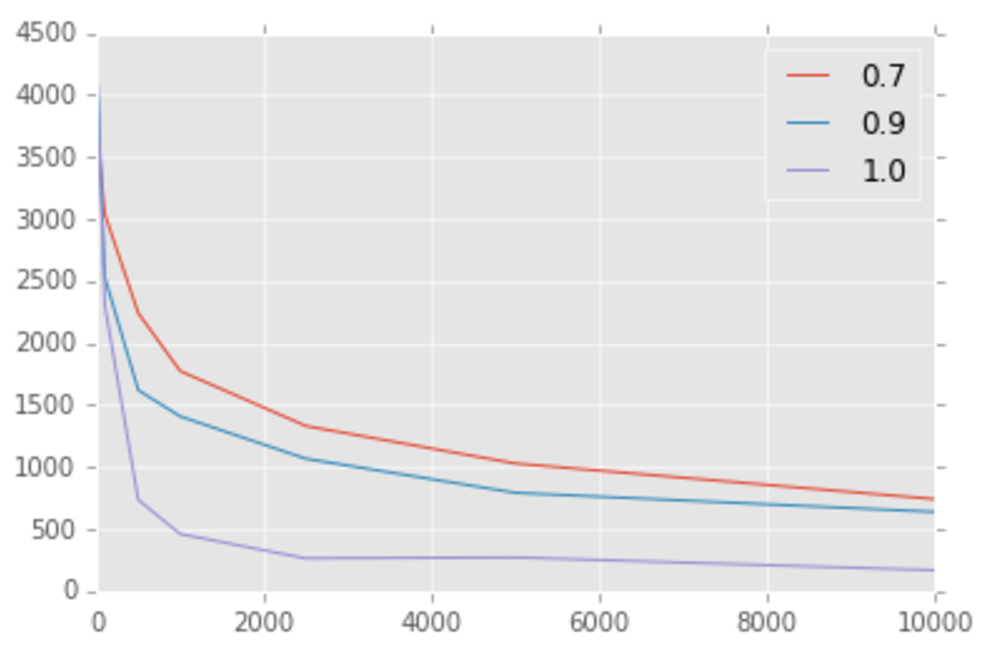
\includegraphics[width=	7cm]{images/pr_100}
\hfill
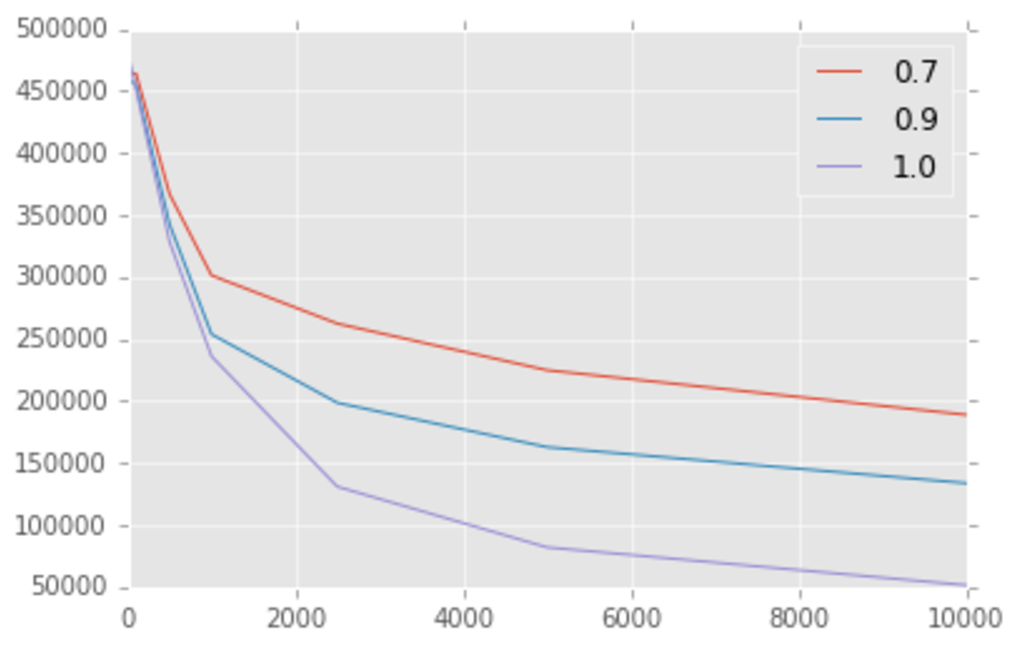
\includegraphics[width=7.2cm]{images/pr_1000}
\caption{Spearman footrule as a function of number of observations, varying preference strengths B. Left plot is V=100, right is V=1000.}
\label{fig:pr_0} 
\end{figure}

We conclude that PrefRank is able to recover a large amount of preference structure.
The quality of the structure recovered increases as the number of pairwise observations increases.
Further, the stronger the underlying preference ($B$), the less data was needed to improve accuracy.
These results are unsurprising but bode well.
More work remains to determine under what circumstances and for what specific types of preference does PrefRank perform better.

\subsection{Prototype}

The complexity of the algorithms discussed above are all, in some form, $O(f(n))$.
Finding some way of reducing $n$ would allow all of these techniques to be applied more quickly.

\bigskip

One way to reduce $n$ would be to identify elements of $V$ which are closely related, and to collapse them into more general ``categories'' or ``prototypes,'' which can be treated as though they were single nodes in a graph.
\citet{rosch:1973} provides theoretical justification for this approach, arguing that human cognition utilizes abstract ``prototypes'' in order to reason heuristically about the world.
Identifying these prototypes is conceptually similar to identifying other types of graphical structures, such as communities in social networks.

Community-finding is a major problem in computer science, and much work has been done on this problem.
We present \textbf{Prototype}, an extension of the Mixed-Membership Stochastic Blockmodel (MMSB) of \cite{airoldi:2008} designed to identify such prototypes among a large set of items.

This is a ``Bayesian model'' in that we first assert a model for our data, in which latent factors (hidden variables) interact and ultimately bring about the data we observe.
Inference in this model amounts to learning the optimal (``posterior'') values of these hidden variables, based on the data.

\subsubsection{Model Specification}

In this model, we assume each item is perceived as a mixture of one or more abstract ``prototypes''.
We then assume there is a fixed ``interaction matrix'' $B$, governing preferences between prototypes, where $B_{gh}$ indicates that probability that an item of prototype $h$ is preferred over an item of prototype $g$.

\bigskip

The generative process is as follows:
\begin{itemize}
	\item For items $p \in V$:
	\begin{itemize}
		\item Draw a $K$-dimensional membership vector $\pi_p \sim Dirichlet(\alpha)$.
	\end{itemize}
	\item For each observation $x_n = (p_n, q_n, y_n) \in X$:
	\begin{itemize}
		\item Draw item type $z_{p_n \rightarrow q_n} \sim Multinomial(\pi_{p_n})$
		\item Draw item type $z_{q_n \rightarrow p_n} \sim Multinomial(\pi_{q_n})$
		\item Draw $y_n \sim Bernoulli(z_{p_n \rightarrow q_n}^TBz_{q_n \rightarrow p_n})$
	\end{itemize}
\end{itemize}


Prototype extends the work of \citet{airoldi:2008} by imposing symmetric structure on the matrix $B$.
Specifically, we enforce that $B_{gh} = 1-B_{hg} \; \forall g,h$ (note that this implies $B_{gg}= 0.5 \; \forall g$).
Unlike other mixed-membership stochastic blockmodels, which emphasize intra-community connective patterns, our model exclusively considers inter-community connective patterns.

This model does not attempt to learn distinct preferences per entity.
This was intentional, as this model is attempting to capture and represent preference in aggregate.
That said, this work could be extended by learning a different interaction matrix $B$
per user.
We leave this for future work.

\subsubsection{Inference}

Our goal is to learn posterior values for $\pi_p, z_{p_n \rightarrow q_n}, z_{q_n \rightarrow p_n}$, and $B$.
$\pi_p, z_{p_n \rightarrow q_n}$, and $z_{q_n \rightarrow p_n}$ are random variables, and we will learn posterior values via mean-field variational inference (\cite{wainwright}, \cite{blei:2016}).
$B$ is a matrix of parameters, and so we learn posterior values via variational Expectation-Maximization.

\bigskip

We first assume the following posterior ``$q$'' distributions:

\begin{itemize}
	\item $q(\pi_p) \sim Dirichlet(\gamma_p)$
	\item $q(z_{p_n \rightarrow q_n}) \sim Multinomial(\phi_{p_n \rightarrow q_n})$
	\item $q(z_{q_n \rightarrow p_n}) \sim Multinomial(\phi_{q_n \rightarrow p_n})$
\end{itemize}

The essence of variational inference (specifically coordinate-ascent VI) is that we can learn the optimal distribution of each variable \textit{given the other variables}.
We iterate over the variables, updating their distributions in turn, with each iteration bringing the $q$ distributions closer to the true posterior.

The update equations are as follows:

\[
\hat{\gamma_{p,k}} = \alpha + \sum_{n \in N} \mathbbm{1}(p = p_n)\phi_{p_n \rightarrow q_n,k} + \sum_{n \in N} \mathbbm{1}(p = q_n)\phi_{q_n \rightarrow p_n,k}
\]

\[
\hat{\phi_{p_n \rightarrow q_n,g}} \propto exp\bigg\{\mathbb{E}_q\big[log(\pi_{p,g})\big] + \sum_{h}\phi_{q_n \rightarrow p_n,h}\mathbb{E}_q\big[logp(y_n|B_{gh})\big]\bigg\}
\]

\[
\hat{\phi_{q_n \rightarrow p_n,h}} \propto exp\bigg\{\mathbb{E}_q\big[log(\pi_{q,h})\big] + \sum_{g}\phi_{p_n \rightarrow q_n,g}\mathbb{E}_q\big[logp(y_n|B_{gh})\big]\bigg\}
\]

\[
\hat{B_{gh}} = \frac{
\sum_{n \in N} \phi_{p_n \rightarrow q_n, g} \phi_{q_n \rightarrow p_n, h} y_n + \phi_{p_n \rightarrow q_n, h} \phi_{q_n \rightarrow p_n, g}(1-y_n)
}{
\sum_{n \in N} \phi_{p_n \rightarrow q_n, g} \phi_{q_n \rightarrow p_n, h} + \phi_{p_n \rightarrow q_n, h} \phi_{q_n \rightarrow p_n, g}
}
\]

\bigskip

Additional details of these derivations are given in Appendix \ref{sec:mmsb_appendix}.
Every iteration of the CAVI algorithm has complexity $O(NK^2 + VK)$, again much slower than the linear-time methods.

\subsubsection{Empirical Results}

We evaluated Prototype in three ways: on simulated data, on film review data, and on survey data.
Additional information on these data sources can be found in Appendix \ref{sec:datasets}.

\bigskip

\textbf{Simulations}

\bigskip

In order to validate our implementation and the validity of the model, we fit our MMSB to simulated data.
For small-to-medium sized graphs, our implementation recovers (with some variation) the true prototype distributions $\pi$ and interaction matrix $B$, given enough observations. See Figures \ref{fig:pi_v_gamma} and \ref{fig:interactions_med}.

\bigskip

\textbf{MovieLens Data}

\bigskip

Given that the MovieLens dataset we work with is constructed based on the
user ratings, the preferences we observe for a single user must be transitive.
As such, for a single user, we expect to be able to learn five ``prototypes'', 
each corresponding to a different rating, with the
interaction matrix $B$ to encoding a transitive ordering among these ratings.
We find that this occurs: when setting $K=5$, the model 
learns a strict ordering among the prototypes, and is able to correctly predict 
this user preferences with $98\%$ accuracy on the heldout dataset (Figure \ref{fig:interactions_movie}).  

With multiple users, we are no longer guaranteed a single shared transitive
ordering.
We see in Figure \ref{fig:acc_movies} that the heldout accuracy of the
MMSB plateaus at around $76\%$ when trained on the data from 30 users.
Adding more prototypes, beyond $K=4$, does not improve the
performance of the model. This suggests that the model is simply assigning each
movie to the prototype corresponding to its average rating; thus, having more
than 5 prototypes is not useful.

\bigskip

\textbf{Survey Data}

\bigskip

We fit Prototype to a survey of beer preferences, first considering only the answers from the single opinionated user.
We fit the model to 900 training observations, and measured predictive accuracy on the remaining 344.
We varied K, the number of prototypes, from 1 to 15, but found that predictive accuracy was very stable for K > 1, hovering around 78\%.
With $K=3$, our model learned a transitive ordering of preferences among prototypes. See Figure \ref{fig:interactions_beer}.

We next considered the answers coming from all other participants.
We fit the model to 150 training observations and measured accuracy on the remaining 74.
We varied K in the same way as before, and observed both more variable and overall weaker predictive accuracy, rarely surpassing 60\%.
We conclude that this model is capable of capturing prototype interaction structure, but it will not perform well given small samples, weakly structured, or very noisy data.


\begin{figure}
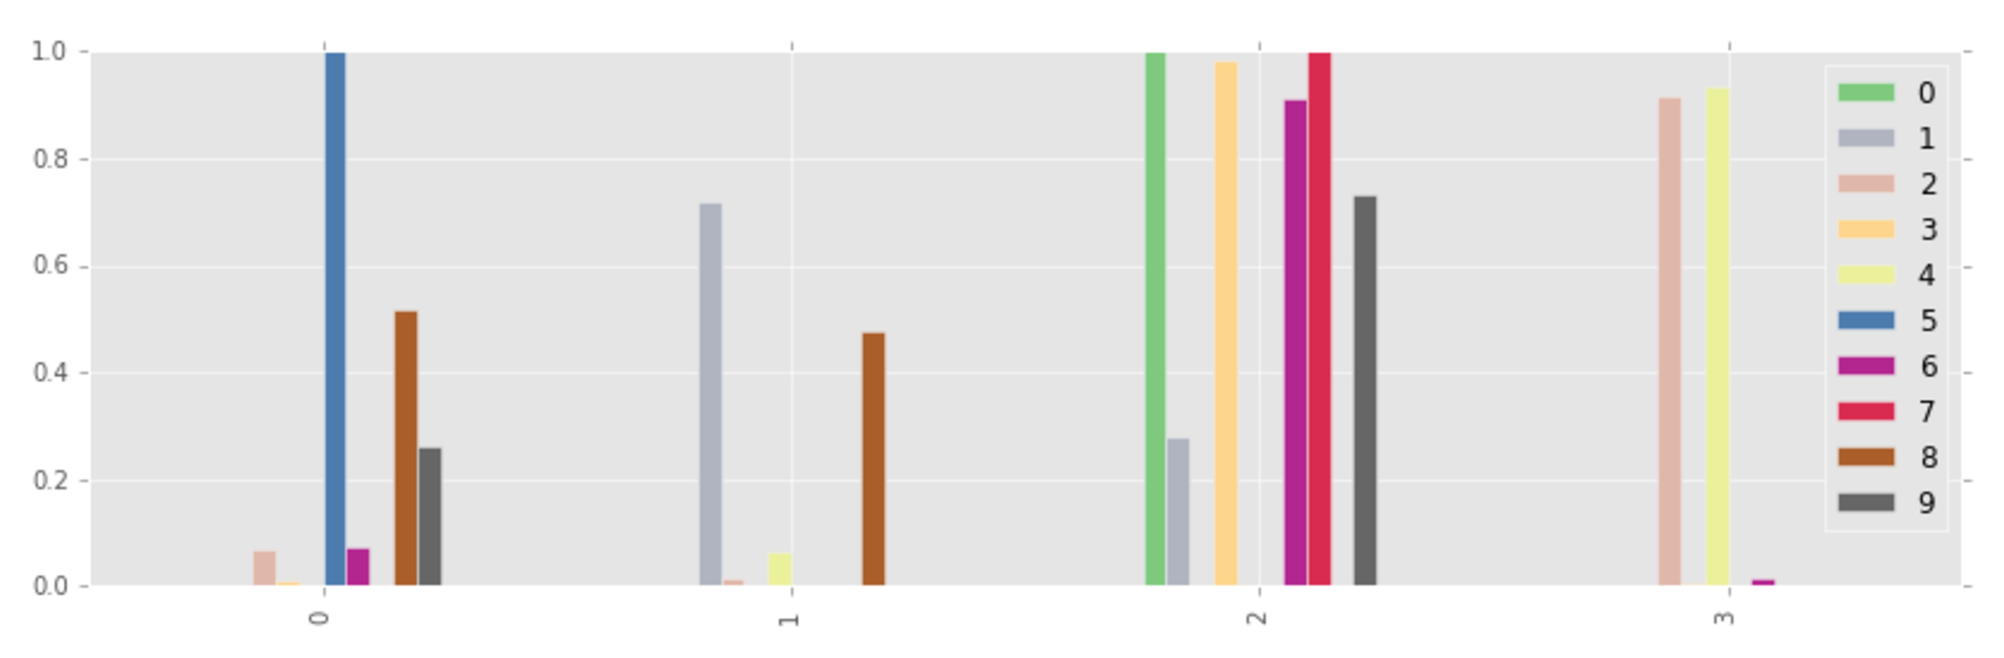
\includegraphics[width=\textwidth]{images/pi}
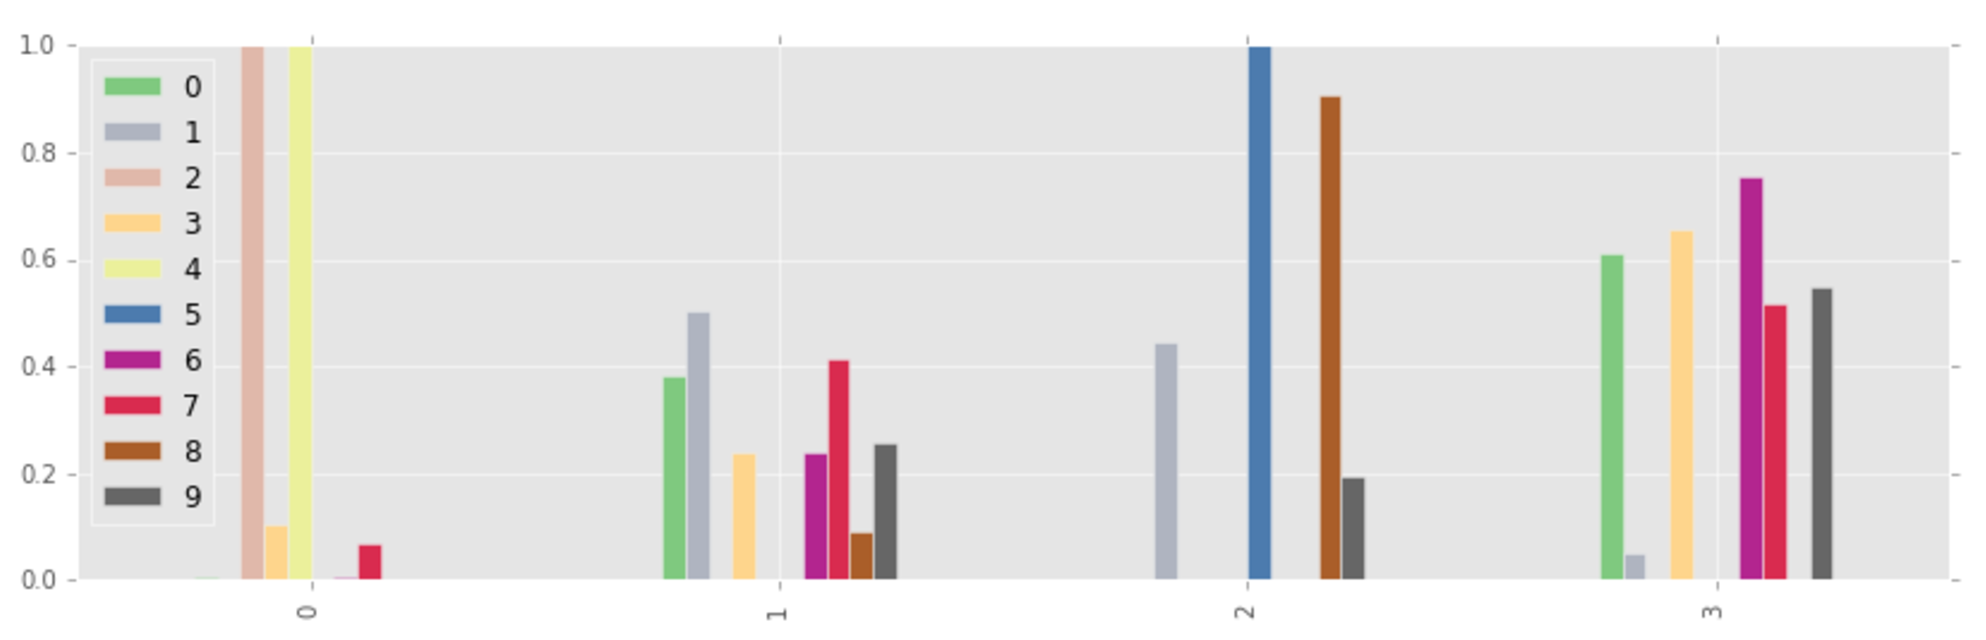
\includegraphics[width=\textwidth]{images/gamma}
\caption{True (top) vs. recovered (bottom) prototype assignments, K=4, V=10, N=10000. We see how the model has correctly grouped the items into their prototypes. Note the label-switching --- this illustrates the multi-modal nature of the joint probability distribution.}
\label{fig:pi_v_gamma} 
\end{figure}


\begin{figure}[!htb]
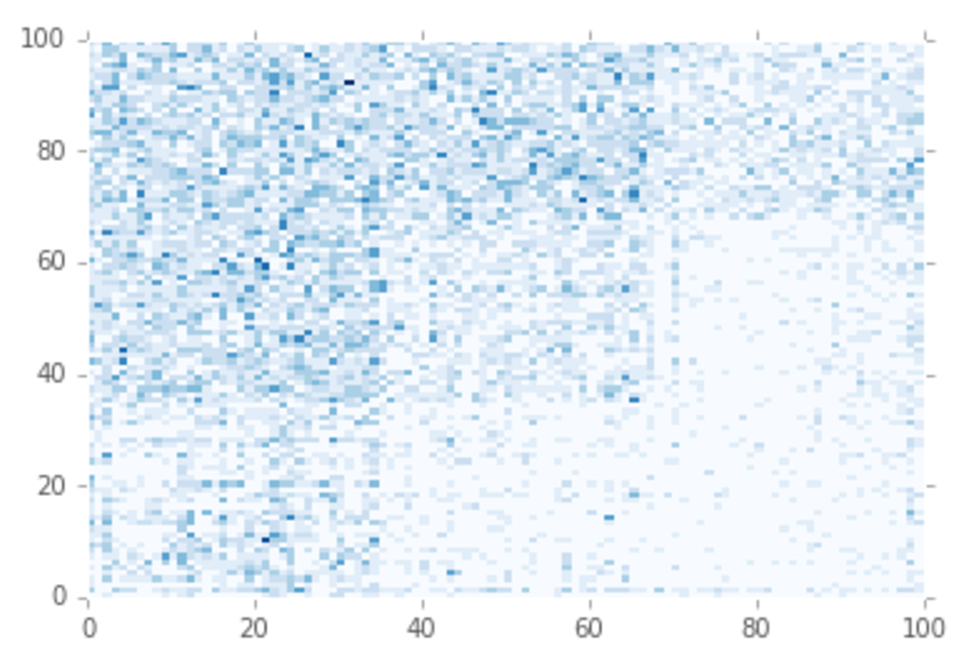
\includegraphics[width=	7cm]{images/10k_5a_95b}
\hfill
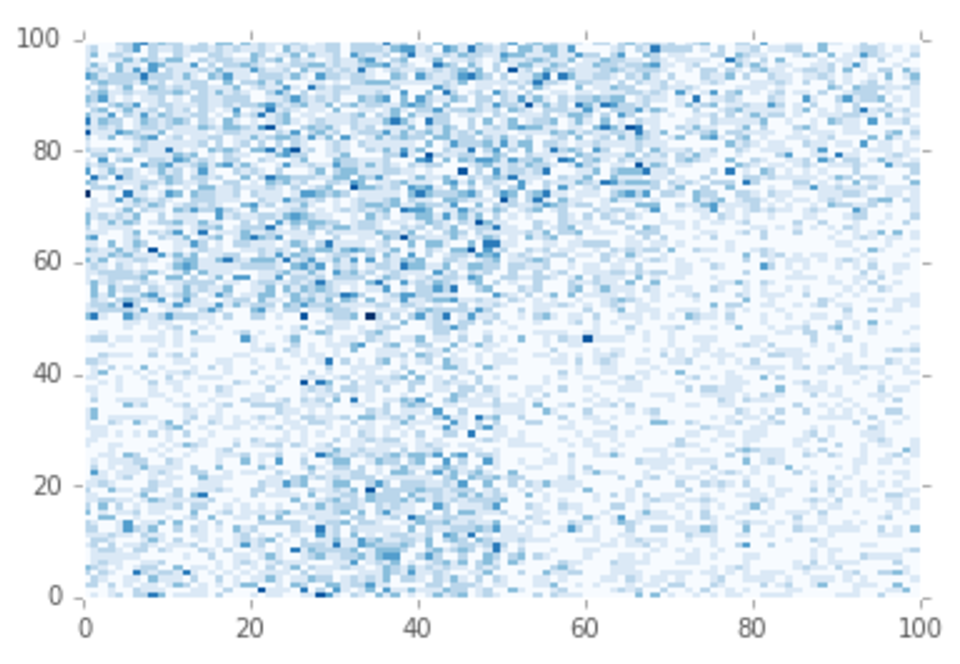
\includegraphics[width=7cm]{images/10k_5a_8b}
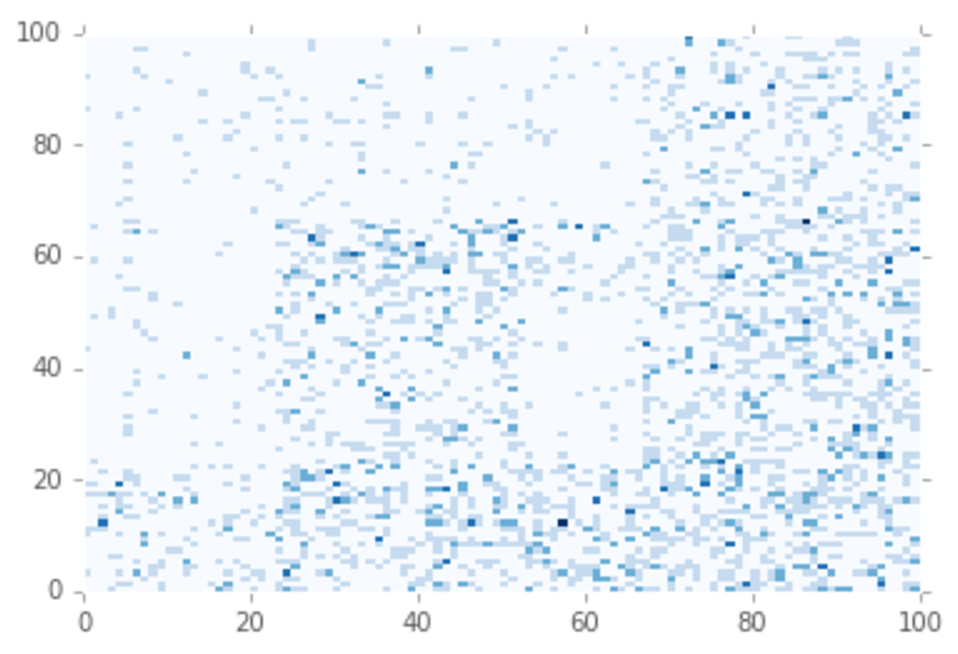
\includegraphics[width=	7cm]{images/2k_5a_95b}
\hfill
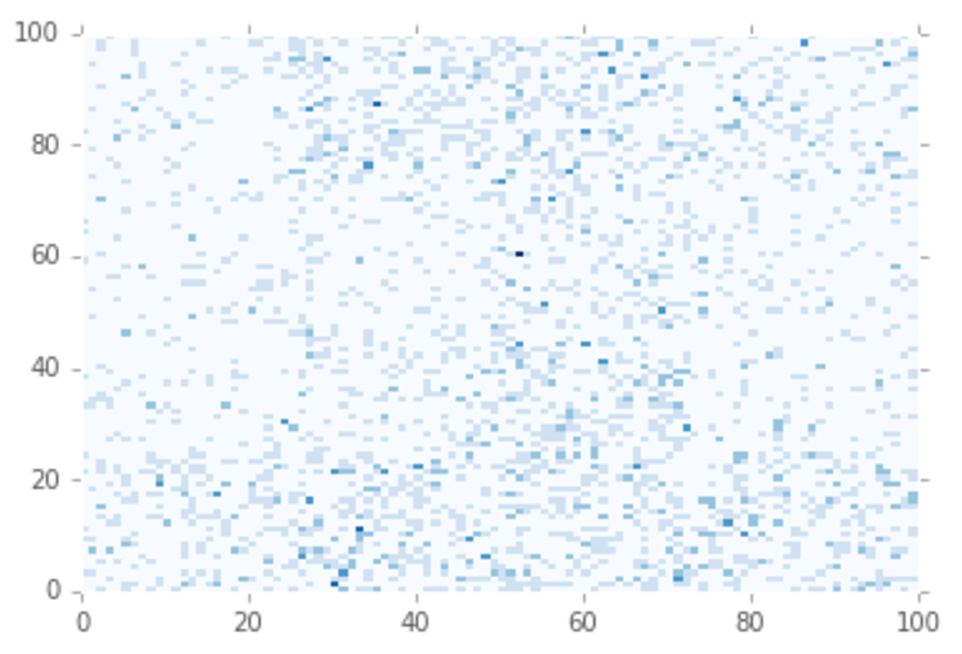
\includegraphics[width=7cm]{images/2k_5a_8b}
\caption{Simulated interaction matrix, items sorted by most likely prototype, K=4, V=100 for all models. Top to bottom: N=1000, 2500. Left to right: B = .95, .8. The visible blocks show that items coming from similar prototypes interact in similar ways to items coming from other prototypes. The diagonal is gray, indicating that intra-prototype comparisons are 50/50 chance.}
\label{fig:interactions_all} 
\end{figure}


\begin{figure}
\centering
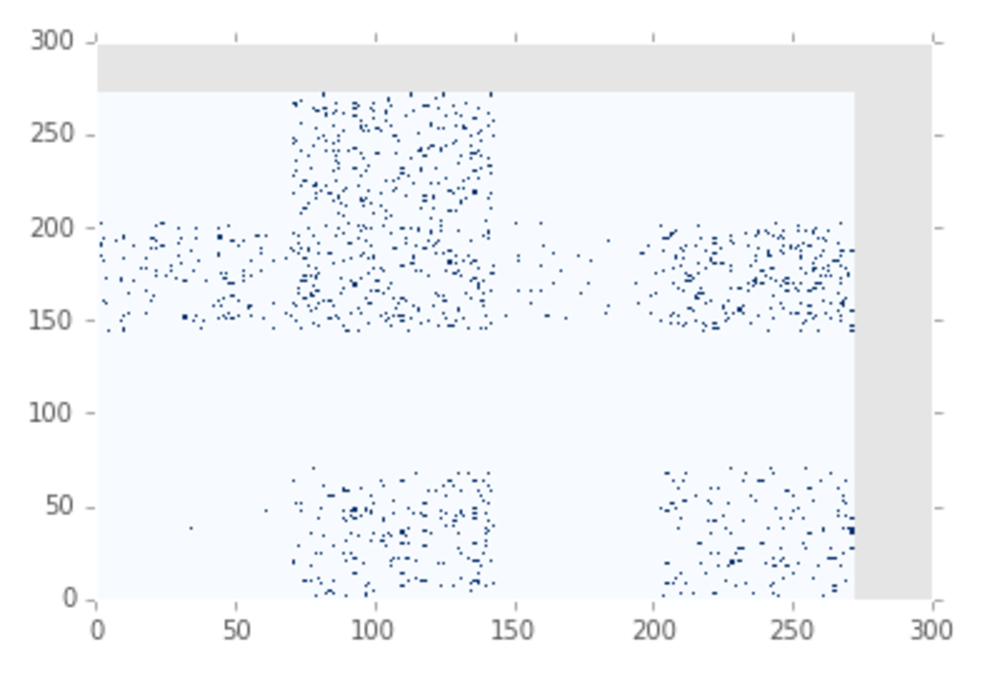
\includegraphics[width=10cm]{images/interactions_movie}
\caption{Movie interaction matrix, one user, items sorted by most likely prototype, K=5, V=272, N=1499}
\label{fig:interactions_movie} 
\end{figure}

\begin{figure}
\centering
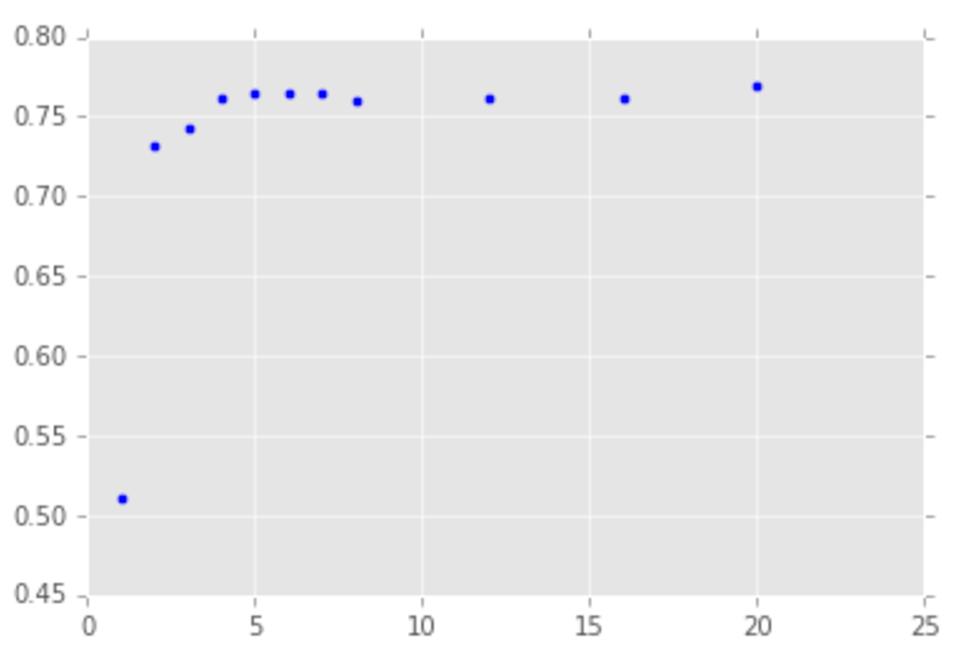
\includegraphics[width=10cm]{images/acc_movies}
\caption{Predictive accuracy against held-out data, 200 films and 20 users, function of number of prototypes $K$. Accuracy plateaus at $K = 4$, suggesting that the model is assigning each movie to a prototype corresponding to an average rating.}
\label{fig:acc_movies} 
\end{figure}


\begin{figure}
\centering
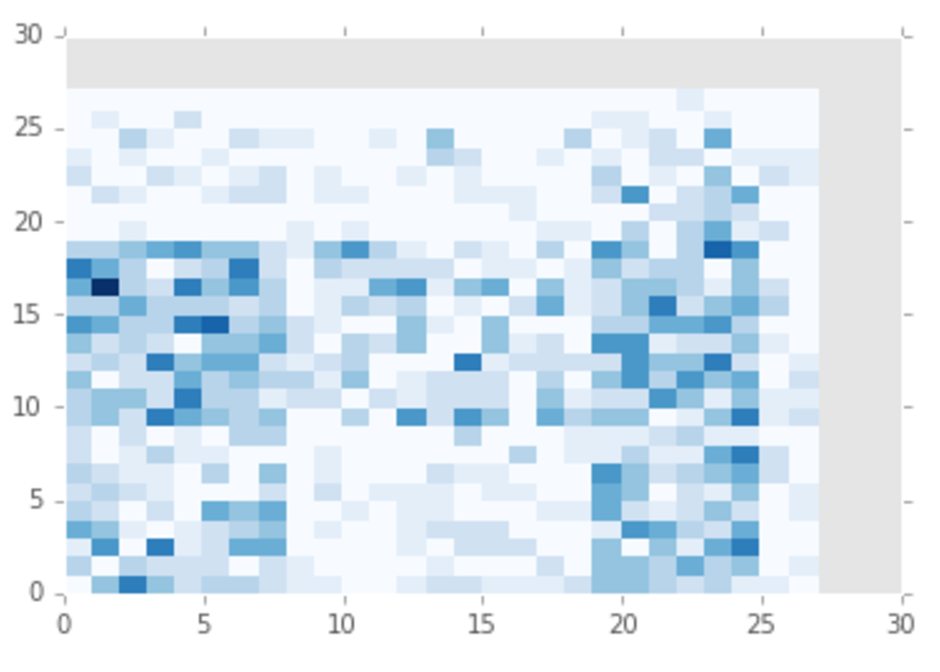
\includegraphics[width=9cm]{images/interactions_beer}
\hfill\raisebox{3cm}{
\begin{tabular}{ | c | c c c | }
\hline
& 0 & 1 & 2 \\ 
\hline
0 & 0.50 & 0.10 & 0.11 \\
1 & 0.90 & 0.50 & 0.89 \\
2 & 0.89 & 0.11 & 0.50 \\
\hline
\end{tabular}
}
\caption{Interaction matrix (left) and B matrix (right) for beer preferences, one user, items sorted by most likely prototype, K=3, V=27, N=1244. We see a transitive ordering of the three prototypes ($1 < 2 < 0$).}
\label{fig:interactions_beer} 
\end{figure}